\documentclass[tikz,border=4mm]{standalone}

\usepackage{fontspec}
\usepackage{amsmath}
\usepackage{unicode-math}
\usepackage{tikz}

\usetikzlibrary{arrows.meta,calc,positioning}

% Compile with LuaLaTeX or XeLaTeX.
\setmainfont{STIX Two Text}
\setmathfont{STIX Two Math}

% Keep the visual language of the original figure, but use it sparingly.
\colorlet{mappingcolor}{blue!58!black}
\colorlet{geometrycolor}{blue!62!black}
\colorlet{fieldcolor}{red!72!black}

\tikzset{
  reference line/.style={black!88, line width=1pt},
  interpolation arrow/.style={
      line width=0.9pt,
        -{Latex[length=2.2mm,width=1.55mm]}
    },
  row label/.style={
      anchor=east,
      font=\normalsize
    }
}

\begin{document}

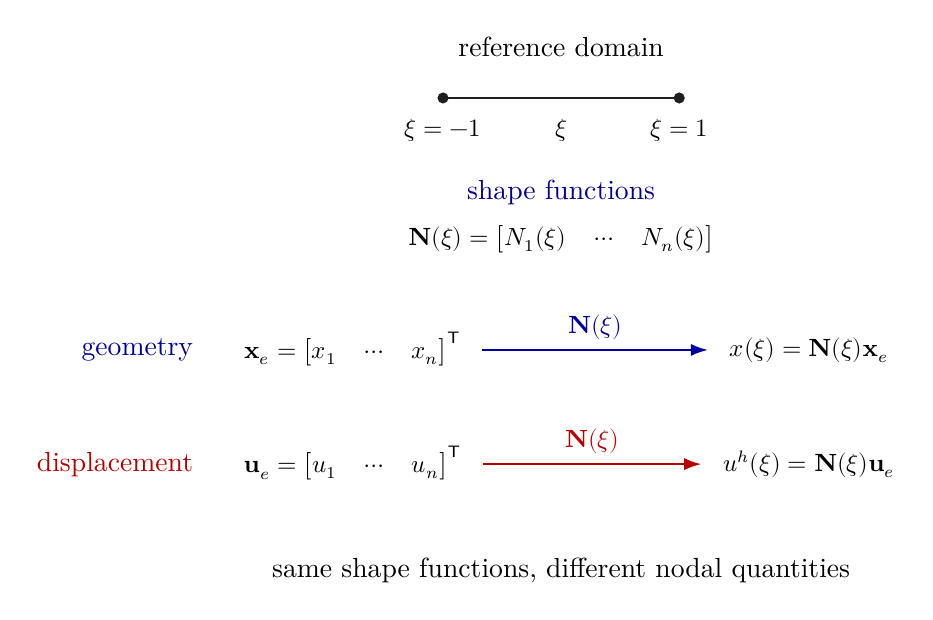
\begin{tikzpicture}[font=\small]

  % ------------------------------------------------------------------
  % Reference domain and common interpolation basis.
  % ------------------------------------------------------------------
  \node[font=\normalsize] at (6.2,6.50) {reference domain};

  \coordinate (rL) at (4.70,5.85);
  \coordinate (rM) at (6.20,5.85);
  \coordinate (rR) at (7.70,5.85);

  \draw[reference line] (rL) -- (rR);
  \fill[black!88] (rL) circle[radius=2pt];
  \fill[black!88] (rR) circle[radius=2pt];

  \node[anchor=north] at ($(rL)+(0,-0.14)$) {$\xi=-1$};
  \node[anchor=north] at ($(rM)+(0,-0.14)$) {$\xi$};
  \node[anchor=north] at ($(rR)+(0,-0.14)$) {$\xi=1$};

  \node[text=mappingcolor, font=\normalsize] at (6.20,4.65)
  {shape functions};

  \node at (6.20,4.05) {$\displaystyle
      \mathbf N(\xi)
      =
      \begin{bmatrix}
        N_1(\xi) & \cdots & N_n(\xi)
      \end{bmatrix}
    $};

  % ------------------------------------------------------------------
  % Two parallel uses of exactly the same interpolation basis.
  % ------------------------------------------------------------------
  \node[row label, text=geometrycolor] at (1.65,2.65) {geometry};

  \node (xdata) at (3.55,2.65) {$\displaystyle
      \mathbf x_e=
      \begin{bmatrix}
        x_1 & \cdots & x_n
      \end{bmatrix}^{\mathsf T}
    $};

  \node (xresult) at (9.35,2.65) {$\displaystyle
      x(\xi)=\mathbf N(\xi)\mathbf x_e
    $};

  \draw[interpolation arrow, geometrycolor]
  ($(xdata.east)+(0.15,0)$) --
  node[above, text=geometrycolor, font=\small] {$\mathbf N(\xi)$}
  ($(xresult.west)+(-0.15,0)$);

  \node[row label, text=fieldcolor] at (1.65,1.20) {displacement};

  \node (udata) at (3.55,1.20) {$\displaystyle
      \mathbf u_e=
      \begin{bmatrix}
        u_1 & \cdots & u_n
      \end{bmatrix}^{\mathsf T}
    $};

  \node (uresult) at (9.35,1.20) {$\displaystyle
      u^h(\xi)=\mathbf N(\xi)\mathbf u_e
    $};

  \draw[interpolation arrow, fieldcolor]
  ($(udata.east)+(0.15,0)$) --
  node[above, text=fieldcolor, font=\small] {$\mathbf N(\xi)$}
  ($(uresult.west)+(-0.15,0)$);

  % ------------------------------------------------------------------
  % Single concluding message.
  % ------------------------------------------------------------------
  \node[font=\normalsize] at (6.20,-0.15)
  {same shape functions, different nodal quantities};

\end{tikzpicture}

\end{document}
